
\begin{algorithm}[!t]
\small
\caption{Label propagation algorithm}
\label{alg:SV_ALG}
\begin{algorithmic}[1]
\Require {$G=(V,E)$}

\State Initialization ;
\For {each $v\in V$}
\State	$CC[v]=v; CCp[v]=v$;
\EndFor

\State $NumChange=|V|$
\While{$NumChange>0$};
\State $NumChange\leftarrow 0$
\State MemCpy($CCp$,$CC$,$|V|$)
\For {each $v\in V$}
\For {each $u\in E(v)$}

\If {$CCp[u]<CC[v]$}
\State $CC[v]\leftarrow CCp[u]$
\State NumChanges = NumChanges+1;
\EndIf

\EndFor
\EndFor

\EndWhile 


\end{algorithmic}
\end{algorithm}
%

Connected components are widely used in graph analytics as these represents subgraphs in the entire 
graph that all vertices are connected. While connected components can not imply the level of 
significance of a vertex, having connected components can be useful for community detection, 
centrality analytics, and for streaming graph analytics.  
Several recent studies show that many real-world social networks may have one connected component 
that includes rougly $90\%$ of the vertices \cite{leskovec2009community,strogatz2001exploring}. 
While many vertices are part of the large connected component, they are not tighlty bound to this 
component and are typically on the ``outskirts'' of this component.

To deal with the increased sizes of graphs numerous parallel algorithms have been designed. One of 
the mostly widely used algorithms is that of Shiloach-Vishkin \cite{ShiloachVishkin}. Variations 
of Shiloach-Viskin can be found in LIGRA \cite{ligra} for the CPU, Gunrock for the GPU 
\cite{gunrock}, and a scalable distributed implementation \cite{flick2015parallel}.	
While this algorithm offers a parallel formulation for connected components, it can also be 
implemented sequentially or used with a single thread as was done in \cite{greenbranchavoiding} for 
figuring out the cost of hardware branch prediction accuracy for graph algorithms. 

\subsection*{Shiloach-Vishkin (~\sv) algorithm for Connect components}

In our current work we augment the ~\sv algorithm to support fault tolerant execution. The ~\sv 
algorithm is a label-propagation algorithm where a label of vertex inside the 
connected component is propagated to the remaining vertice of that component. Many formulations 
use the label of the vertex with either the minimal or maximal id within a component as the value 
that is propagate. We to use this formulation and propagate the smallest id within the connected 
component. Pseudo code for this algorithm can be found in ~\refAlgorithm{alg:SV_ALG}. The symbols 
used in this algorithm and the fault tolerant algorithm introduced in the next section can be found 
in \refTable{tab:symbols}.

In the initialization phase, each vertex is placed in its own connected component. From this point 
on, in each iteration of the algorithm vertices inspect the connected component value of their 
neighbors, \CCVAL. If one of the neighbors has a smaller id then the vertex will switch its 
connected component to the one that its neighbor has chosen. \refFigure{fig:svPropagation} depicts 
how the label propagates from its initial state, \refFigure{fig:svPropagation} (a), to its final 
state \refFigure{fig:svPropagation} (e), where the label of the vertex with the smallest id takes 
over all the vertices in the component.  The algorithm terminates when an iteration as completed 
and no vertex has swapped its \CCVAL label.
One of the key findings of \cite{greenbranchavoiding} is 
that the label swapping occurs at a higher rate in the initial iterations. In the advanced 
iteration, the only vertices that have yet to swap their labels are those that are far away from the 
vertex with the smallest id.


The time complexity of the $\sv$ algorithm is as follows. Each iteration requires $O(|V|+|E|)$ 
computations for accessing the connected component array for all vertices and their adadjacencies. 
The number of iterations of the algorithm is bound by $O(log(|V|))$ iterations 
\cite{ShiloachVishkin} using the shortcutting stage of the algorithm. For many real world networks, 
especially small world networks, the number of iterations is bounded by the graph diameter $d$ which 
is the upperbound on how long it would take for a value to propagate from one end of the graph to 
the other. As such, the total time complexity of the algorithm can be written as $O(log(|V|) \cdot 
(|V|+|E|))$ or $O(d \cdot (|V|+|E|))$. We chose the later of these for our analysis. 


\subsubsection*{Observartions}

{\bf 1)} The pseudo code in \refAlgorithm{alg:SV_ALG} uses \CCVAL$^i$ to store the 
connected components after iteration $i$. While it may seem that these arrays are stored for all 
the iterations, in practice it is only necessary to store these for two consecutive 
iterations as the previous ones are not necessary.

{\bf 2)} Upon completion of the algorithm, each vertex is assigned to exactly one connected 
component and this can be found in \CCVAL$^\infty$. Given that our formulation of \sv uses the 
minimal id formulation, we assume that each vertex points to the vertex with the smallest 
id in the connected component. We refer to this as the {\bf final and correct state}.

\begin{table*}
\centering
\footnotesize
\caption{Symbols used in the fault free \sv algorithm and in the new fault tolerant algorithm.}
\begin{tabular}[t]{|l|l|r|}\hline
Symbol & Decription & Size\\\hline\hline
$V$ & Vertices in the graph & O(V)\\\hline
$E$ & Edges in the graph & O(E)\\\hline
$adj(v)$ & Adjacency list for vertex $v\in V$ & \\\hline
\CCVAL & Connected component array & O(V)\\\hline
\CCVAL$^i$ & Connected component array after iteration $i$ & O(V)\\\hline
\CCVAL$^\infty$ & The final connected component mapping upon algorithm completion. & O(V)\\\hline

& Fault free \\
\hline
$H$ &  & O(V)\\\hline
\end{tabular}
\label{tab:symbols}
\end{table*}


\begin{figure*}[t]
\centering
	\subfloat[]{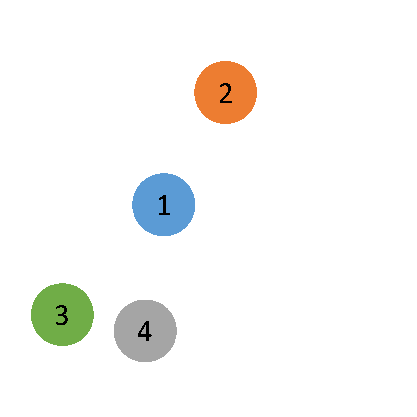
\includegraphics[width=0.2\textwidth]{figure/sv1.pdf}}
	\subfloat[]{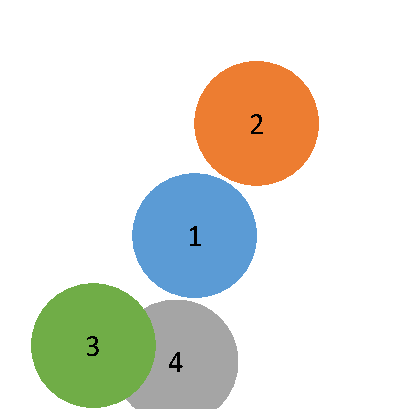
\includegraphics[width=0.2\textwidth]{figure/sv2.pdf}}
	\subfloat[]{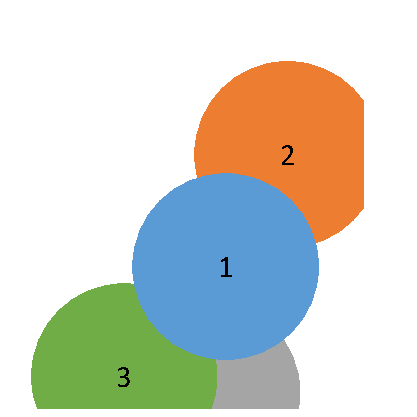
\includegraphics[width=0.2\textwidth]{figure/sv3.pdf}}
	\subfloat[]{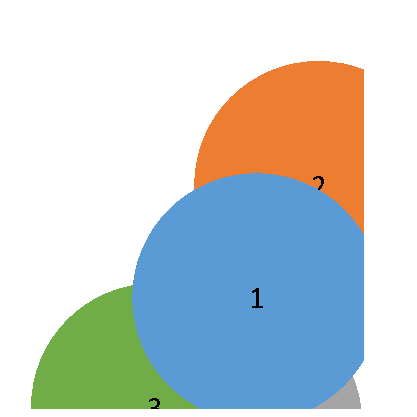
\includegraphics[width=0.2\textwidth]{figure/sv4.pdf}}
	\subfloat[]{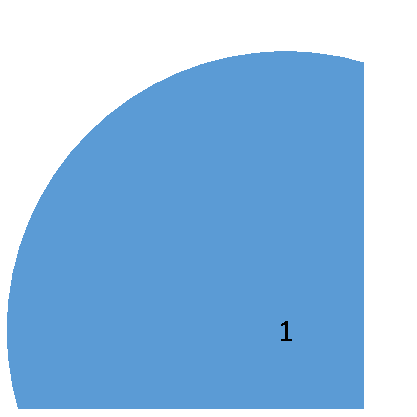
\includegraphics[width=0.2\textwidth]{figure/sv5.pdf}}

  \caption{These sub-figures conceptually show how the connected component id propagates through 
  the graph as time evolves. Subfigures represent snapshots of the algorithm at different times. 
For simplicity, this example assumes that all the shown vertices are connected. Initially the 
number of connected components is equal to the number vertices. (a) Depicts the initial state in 
which each vertex is in its own component. (b)-(d) depict that some vertices belong to the same 
connected component yet may require multiple label updates (in either the same iteration or a 
separate iteration).
	(e) is the final state in which there is a single connected component.}
  \label{fig:svPropagation}
\end{figure*}


  